\section{Benchmark Hiệu Năng và Khả Năng Mở Rộng Overlay}

\subsection{Mục Tiêu Benchmark}
Mục tiêu của benchmark là trả lời câu hỏi:

\begin{quote}
Full mesh broadcast và DHT-based broadcast khác nhau thế nào khi số peer tăng?
\end{quote}

Benchmark này \textbf{không} nhằm chứng minh một chế độ luôn tốt hơn chế độ còn lại. Thay vào đó, nó đánh giá sự đánh đổi giữa \textit{độ trễ chuyển phát trực tiếp} và \textit{khả năng mở rộng số lượng kết nối}:
\begin{quote}
Benchmark này không nhằm chứng minh một chế độ luôn tốt hơn chế độ còn lại. Thay vào đó, nó đánh giá sự đánh đổi giữa độ trễ chuyển phát trực tiếp và khả năng mở rộng số lượng kết nối.
\end{quote}

\subsection{Thiết Lập Benchmark}
Thiết lập thực nghiệm:
\begin{itemize}[leftmargin=2em]
    \item Mỗi peer được chạy như một tiến trình Python độc lập.
    \item Một tiến trình tracker được dùng cho discovery và quản lý membership.
    \item Cả hai chế độ đều chạy trên cùng một máy.
    \item Authentication được tắt hoặc được bỏ qua cho mục đích benchmark.
    \item Benchmark ghi log dạng JSON và Markdown sau mỗi lần chạy.
\end{itemize}

Các biến đầu vào trong ma trận benchmark:
\begin{itemize}[leftmargin=2em]
    \item \texttt{nodes}: 10, 20, \ldots, 100
    \item \texttt{messages}: 20
    \item \texttt{payload}: 256 byte
\end{itemize}

Các chỉ số (metrics) chính được ghi nhận:
\begin{itemize}[leftmargin=2em]
    \item tổng số kết nối giữa các peer
    \item tỷ lệ chuyển phát thành công
    \item số lượng bản sao (duplicate)
    \item độ trễ p50
    \item độ trễ p95
    \item độ trễ lớn nhất
    \item bộ nhớ RSS
\end{itemize}

\subsection{Khả Năng Mở Rộng Kết Nối}
Full mesh yêu cầu mỗi peer kết nối trực tiếp đến mọi peer còn lại, do đó số lượng kết nối trực tiếp tăng theo bậc hai khi số node tăng. Ngược lại, DHT overlay duy trì một tập kết nối overlay nhỏ hơn, và chuyển tiếp bản tin qua lớp overlay thay vì fan-out trực tiếp đến toàn bộ members.

\begin{figure}[H]
\centering
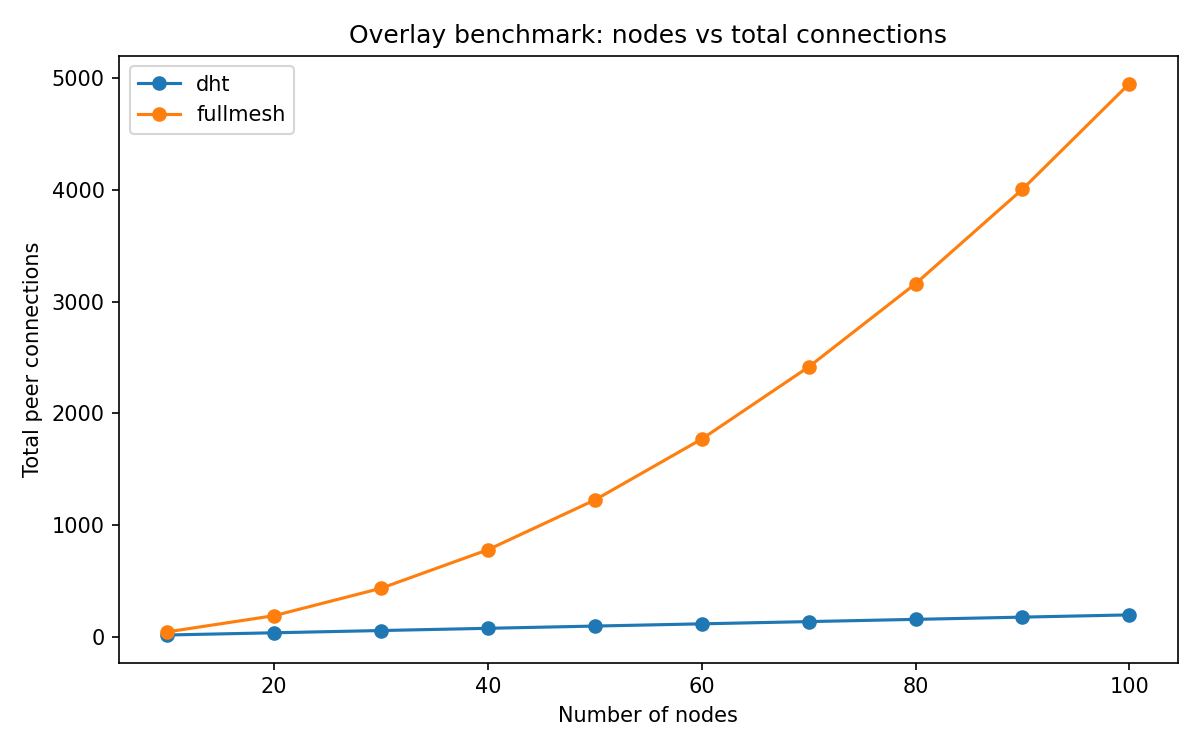
\includegraphics[width=\textwidth]{assets/benchmark-plots/nodes_vs_connections.png}
\caption{Tổng số kết nối trực tiếp khi số node tăng. Full mesh tăng theo bậc hai, trong khi DHT overlay giữ số kết nối trực tiếp ở mức thấp hơn đáng kể.}
\end{figure}

\subsection{Đánh Đổi Về Độ Trễ}
Ở quy mô nhỏ, full mesh thường có độ trễ p95 thấp hơn vì đường truyền là chuyển phát trực tiếp. Khi số node tăng, số lượng kết nối và chi phí quản lý socket của full mesh tăng mạnh, và DHT trở nên cạnh tranh (hoặc tốt hơn) về độ trễ đuôi trong một số cấu hình.

\begin{figure}[H]
\centering
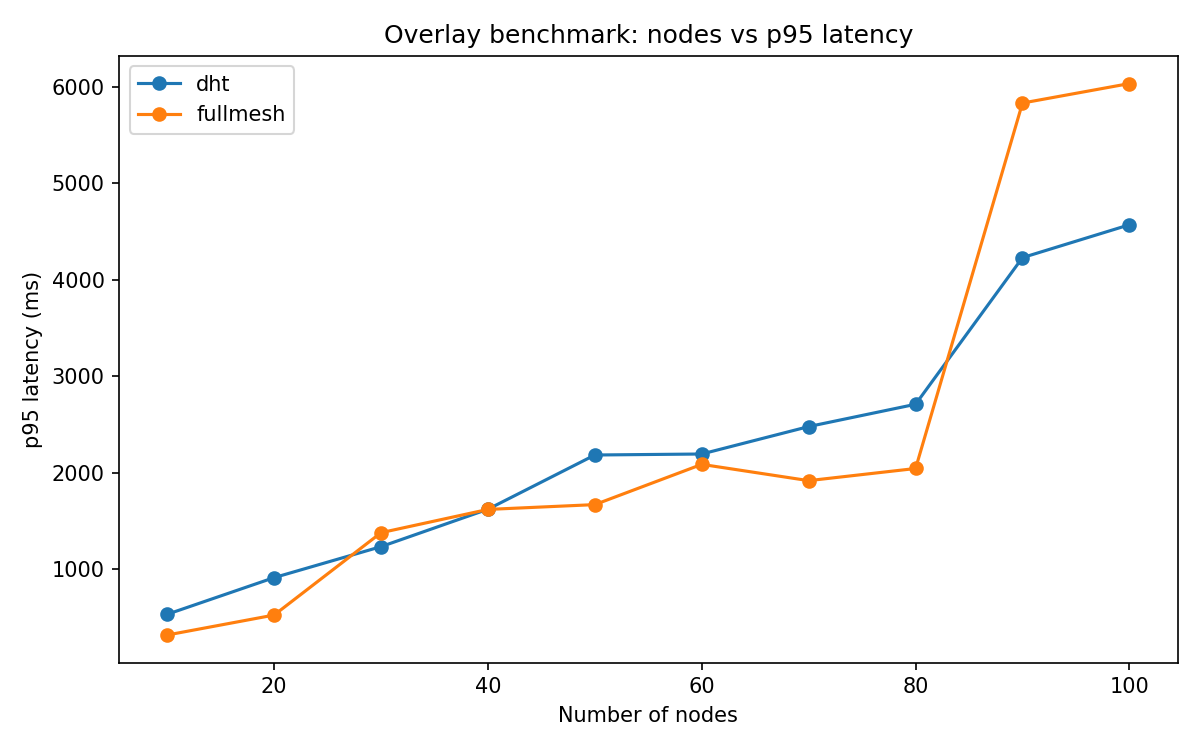
\includegraphics[width=\textwidth]{assets/benchmark-plots/nodes_vs_p95_latency.png}
\caption{Độ trễ đuôi (p95) theo số node. Full mesh có lợi thế chuyển phát trực tiếp ở quy mô nhỏ, còn DHT overlay chấp nhận thêm hop định tuyến để đổi lấy khả năng mở rộng kết nối.}
\end{figure}

\subsection{Độ Tin Cậy và Tính Đúng Đắn Khi Chuyển Phát}
Các lần chạy benchmark đã hoàn tất cho thấy cả hai overlay đều đạt tính đúng đắn khi chuyển phát tốt. Trong các lần chạy đã hoàn thành, hai overlay đều giao đủ số bản tin kỳ vọng với \textbf{không có lỗi chuyển phát} và \textbf{không có bản sao (duplicate)}. Kết quả này bổ sung cho Mục 07: phần xử lý lỗi tập trung vào cơ chế ở mức giao thức/runtime, còn benchmark ở đây kiểm chứng rằng broadcast không tạo bản sao hoặc làm mất bản tin trong điều kiện test.

\begin{figure}[H]
\centering
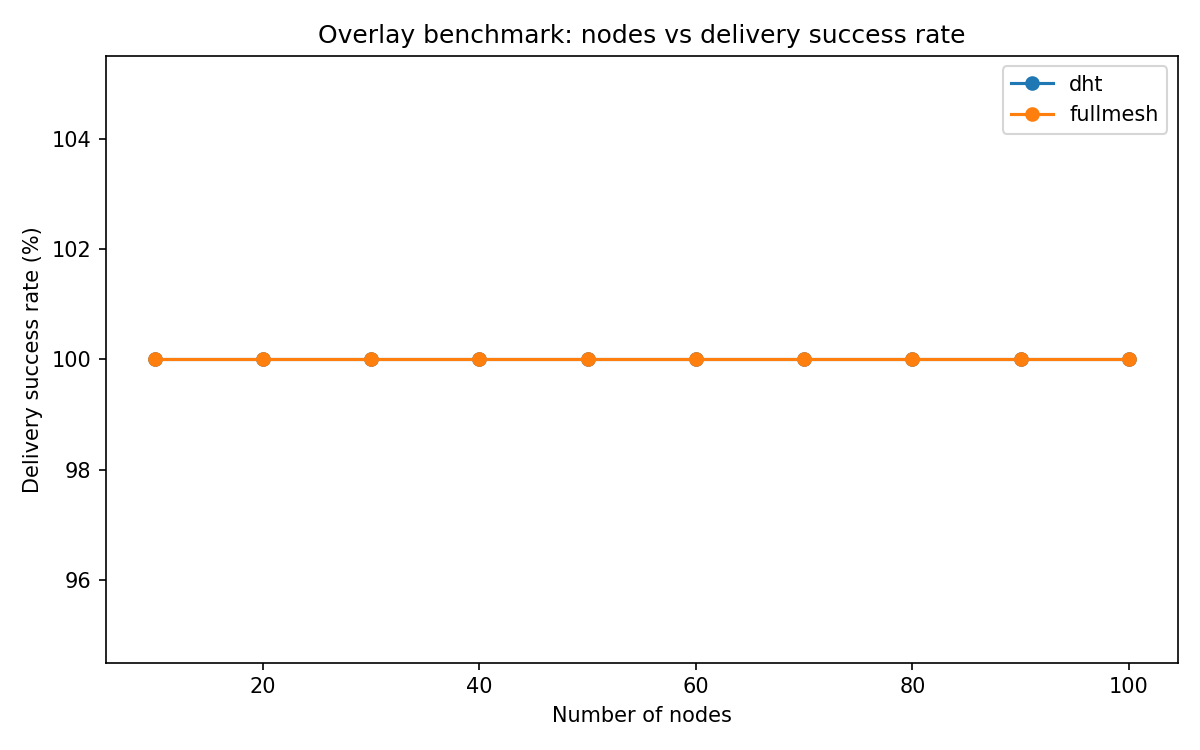
\includegraphics[width=\textwidth]{assets/benchmark-plots/nodes_vs_success_rate.png}
\caption{Tỷ lệ chuyển phát thành công theo số node. Các lần chạy đã hoàn tất cho thấy không mất bản tin và không có bản sao (duplicate).}
\end{figure}

\subsection{Quan Sát Về Bộ Nhớ}
Bộ nhớ RSS quan sát được khá tương đồng giữa hai chế độ vì benchmark khởi tạo một tiến trình Python cho mỗi peer. Do đó, bộ nhớ chủ yếu bị chi phối bởi chi phí runtime theo tiến trình, không chỉ bởi số lượng socket/kết nối.

\begin{figure}[H]
\centering
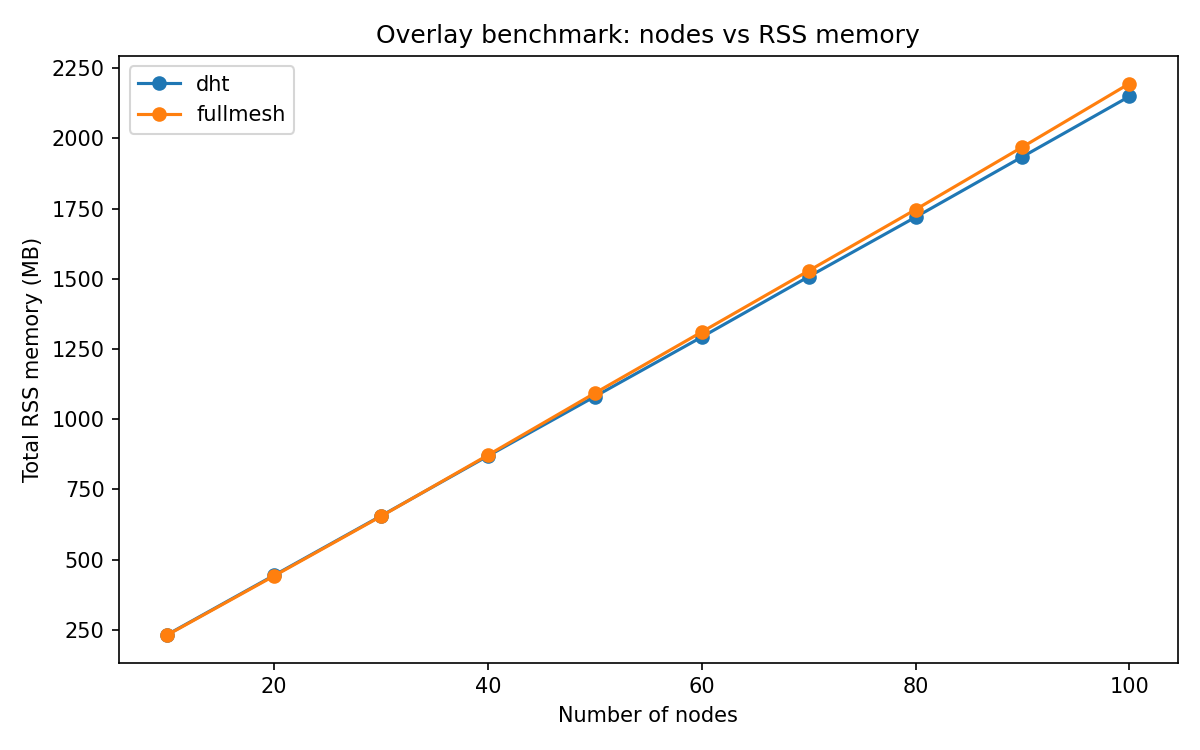
\includegraphics[width=\textwidth]{assets/benchmark-plots/nodes_vs_rss_mb_total.png}
\caption{Tổng bộ nhớ RSS theo số node. Trong benchmark này, bộ nhớ chủ yếu bị chi phối bởi chi phí runtime theo tiến trình.}
\end{figure}

\subsection{Tóm Tắt}
Tóm lại:
\begin{itemize}[leftmargin=2em]
    \item Full mesh đơn giản và hiệu quả về độ trễ ở quy mô nhỏ, nhưng số lượng kết nối tăng rất nhanh khi số node tăng.
    \item DHT thêm chi phí định tuyến (chuyển tiếp qua overlay), nhưng giảm mạnh số kết nối trực tiếp và phù hợp hơn khi cần mở rộng số peer.
\end{itemize}
